	\subsection{PLL: Phase-locked loops}
	\subsubsection{Introducción}
	Los circuitos \textbf{PLL} fueron introducidos a en el año 1960. Sin embargo, su concepto ya había sido probado 30 años atrás pero las limitaciones tecnológicas de la época. Son utilizados en diversas aplicaciones en el área de RF. Se emplean para demodular FM y FSK, acondicionamiento de señales y síntesis de frecuencias. En este trabajo nos dedicaremos a analizar como utilizar un PLL para demodular una señal de FM y a sintetizar una señal cuya frecuencia sea múltiplo de otra. Además estudiaremos el comportamiento del circuito bajo diferentes condiciones.
	
	\subsubsection{Diagrama en bloques de un PLL}
	El PLL consiste de 3 bloques fundamentales:
	
	\begin{enumerate}
		\item  Comparador $\hookrightarrow$ Brinda una señal de error
		\item  Filtro pasa bajos (LPF) $\hookrightarrow$ Promedia la señal de error
		\item  VCO (voltage controlled oscilator) $\hookrightarrow$ Oscilación controlada por la señal de error 
	\end{enumerate}
	
	\begin{figure}[H]
		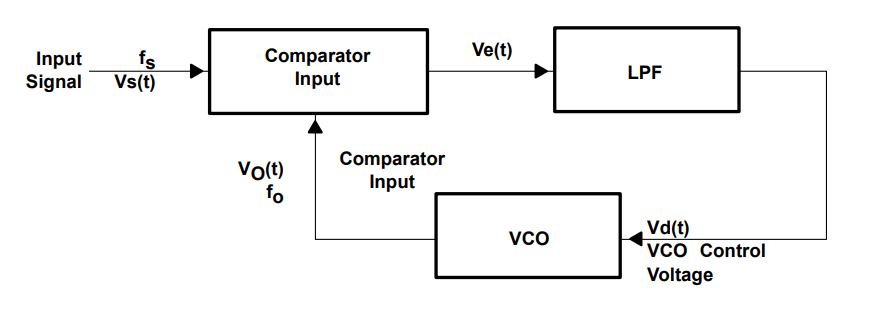
\includegraphics[width=\linewidth]{ImagenesVarias/PLLblockDiagram.PNG}
		\caption{Diagrama en bloques de un PLL}
	\end{figure}
El comparador emite una señal de error proporcional a la diferencia de frecuencia con respecto a la señal de entrada. De no haber entrada (es decir tensión nula) el VCO operara a la frecuencia central ya configurada. La señal de error $V_e(t)$ es filtrada para asegurar que el VCO reciba una señal continua en su entrada. La configuración de retroalimentación busca minimizar la tensión de error. Para esto el VCO ajustara su frecuencia de operación. Por ejemplo, supongamos que la frecuencia central del VCO es $1Khz$ y nuestra entrada opera a $2Khz$. En este caso la señal de error proporcional a dicha diferencia forzara al VCO a aumentar su frecuencia de oscilación. Cuando nuestra frecuencia de entrada se aproxima a la frecuencia de central del VCO se dice que entra al \emph{Rango de captura o enganche}. Al entrar en esta zona y por efecto del circuito de retroalimentación, el VCO sincroniza su frecuencia de oscilación con aquella en la entrada del PLL.


\begin{figure}[H]
	\centering
	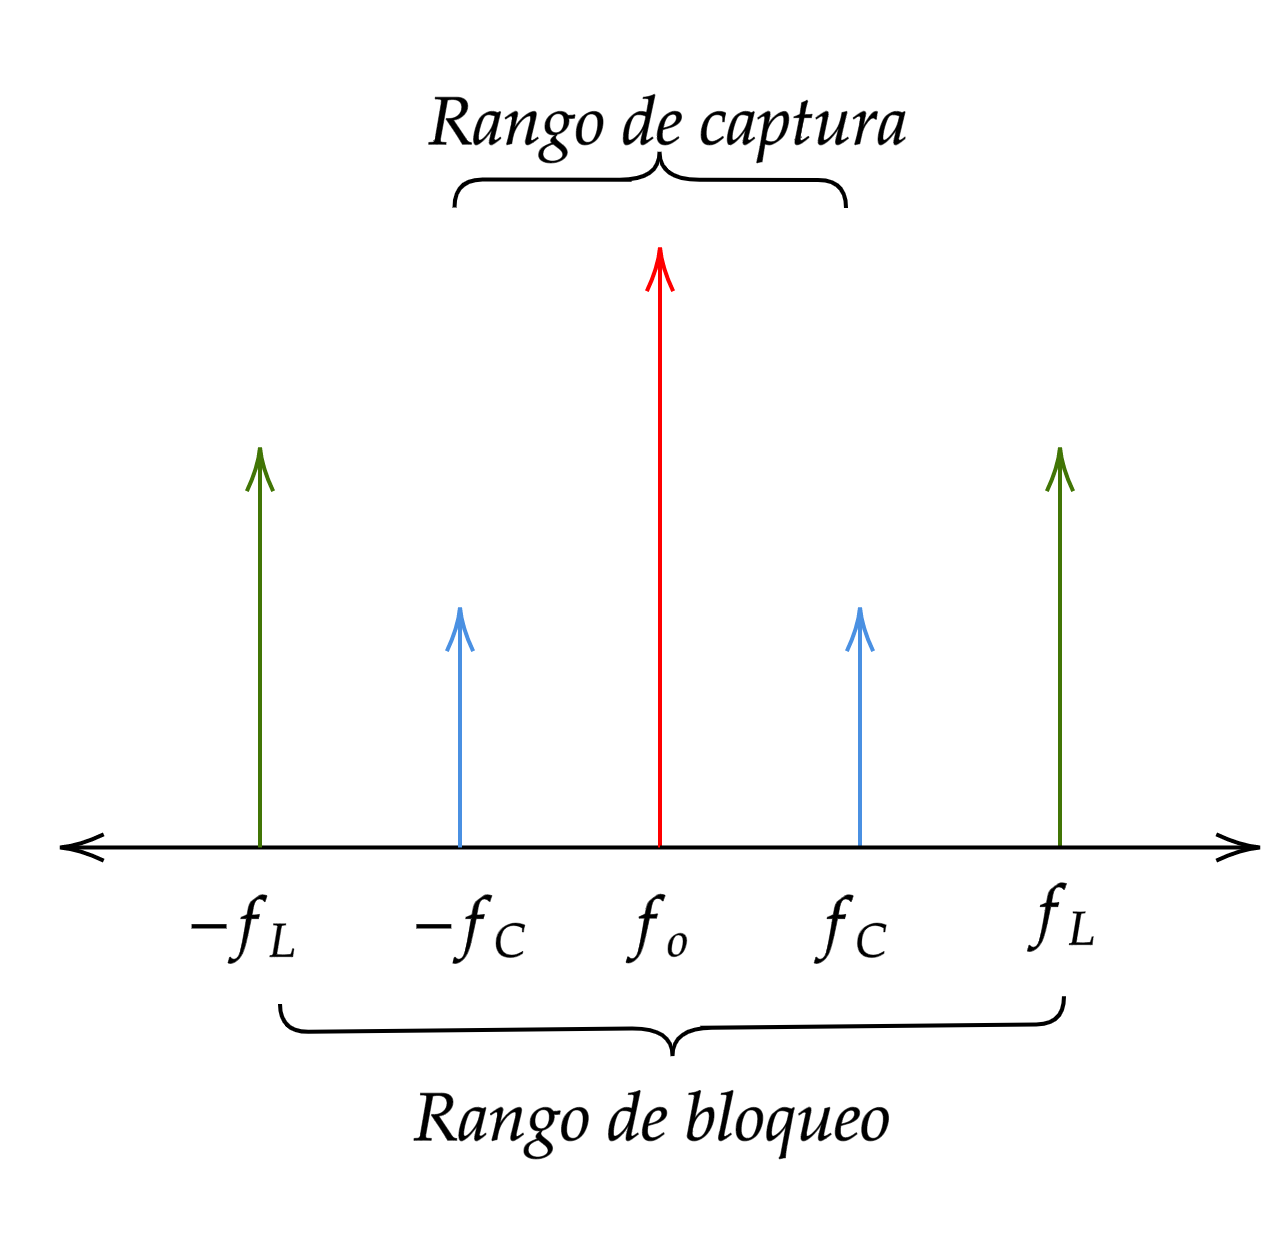
\includegraphics[scale=0.3]{ImagenesVarias/PLL_range2.png}
	\caption{Rango de bloqueo(enganche) y captura}
	\label{blockLockRange}
\end{figure}

Como podemos observar en la figura \ref{blockLockRange}. Existe la ya antes mencionada \textbf{zona de captura}. Una señal que se encuentre en este rango de frecuencias forzara al PLL a sincronizar la frecuencia de oscilación de su VCO interno con la frecuencia de la señal entrante. U na vez dentro de esta zona es posible utilizar el PLL dentro de la llamada \textbf{zona de bloqueo}. En esta zona el PLL mantendrá la frecuencia de oscilación sincronizada. Notemos que el rango de bloqueo es más grande que el rango de captura.

\subsubsection{Diseño y configuración}
El circuito integrado CD4046 puede ser configurado de varias maneras dependiendo de su finalidad.
En la figura \ref{configuraciones} podemos ver los componentes internos del integrado. 

\begin{figure}[H]
	\centering
	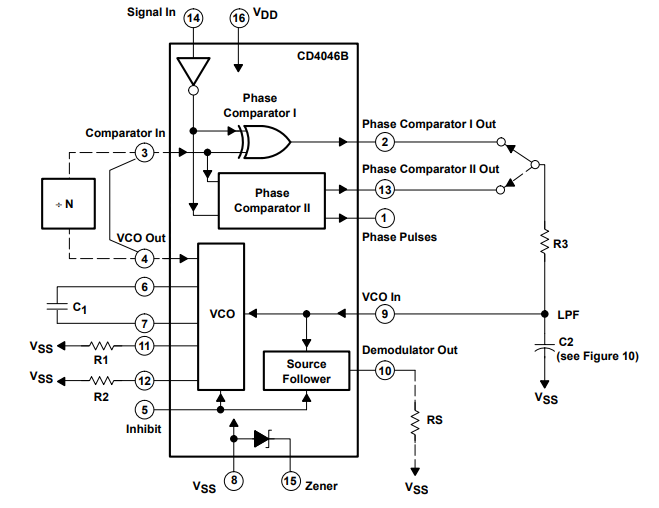
\includegraphics[scale=0.5]{ImagenesVarias/PLL_innerblockdiagram.png}
	\caption{Configuraciones del CD4046 }
	\label{configuraciones}
\end{figure}

En nuestro caso, nos es de interés configurar el PLL de tal forma de obtener un rango de bloque que comience en los $4.5KHz$ y termine a los $96KHz$. Además deseamos poder observar el efecto del rango de captura por lo que este se configurara para capturar frecuencias en un rango de captura dentro del rango de bloque.



\begin{figure}[H]
	\centering
	\includegraphics[scale=0.5]{ImagenesOsciloscopio/Enganchado.png}
	\caption{PLL en funcionamiento siguiendo la frecuencia de la señal de input}
	\label{PLLENGANCHADO1}
\end{figure}



\begin{figure}[H]
	\centering
	\includegraphics[scale=0.5]{ImagenesOsciloscopio/Desengachado.png}
	\caption{PLL desenganchado en la cota superior. En violeta la señal de input, en amarillo la oscilación del VCO no enganchado}
	\label{PLLDESENGANCHADO1}
\end{figure}

\begin{figure}[H]
	\centering
	\includegraphics[scale=0.5]{ImagenesOsciloscopio/DesenganchadoInf.png}
	\caption{PLL desenganchado en la cota inferior. En violeta la señal de input, en amarillo la oscilación del VCO no enganchado}
	\label{PLLDESENGANCHADO1}
\end{figure}






Para alcanzar esta configuración se hizo referencia a la hoja de datos (ver adjunto) de Texas Instruments. \footnote{Durante el desarrollo de este trabajo se encontraron discrepancias en las formulas provistas por los diversos fabricantes. No obstante, coincidían en los circuitos de aplicación planteados}.
En la misma se hace referencia a 4 configuraciones posibles de la cuales solo 1 de ellas nos permite regular el rango de captura de la señal entrante. Las demás establecen un rango de captura de igual ancho que el rango de bloqueo.


\subsubsection{Síntesis de frecuencias}
Los circuitos PLL son utilizados para la síntesis de frecuencias. Esto es de gran utilidad a la hora de construir sintonizadores de radio dado que por ejemplo las emisoras de AM cuentan con un ancho de banda finito y disponible (hay $10KHz$ entre emisoras). Entonces, resulta conveniente un dispositivo que, a partir de una frecuencia de referencia, genere osciladores locales ajustados a la frecuencia de las emisoras para poder captarlas. Esto tiene la ventaja de necesitar un solo oscilador de referencia para sintetizar frecuencias de forma fiable.
Para poder elevar la frecuencia de nuestro sistema primero debemos generar un divisor de frecuencias. A primera vista esto parece ir en contra de nuestro objetivo, aumentarla, sin embargo colocar un divisor de frecuencia entre la salida del VCO y la entrada del comparador en uso forzara al sistema a generar una señal de mayor frecuencia aún dado que el comparador generara un tren de pulsos con mayor contenido de energía que, luego de pasar por el \emph{LPF}, proporcionara al VCO una señal que lo conducirá a incrementar su frecuencia de oscilación.

\begin{figure}[H]
	\centering
	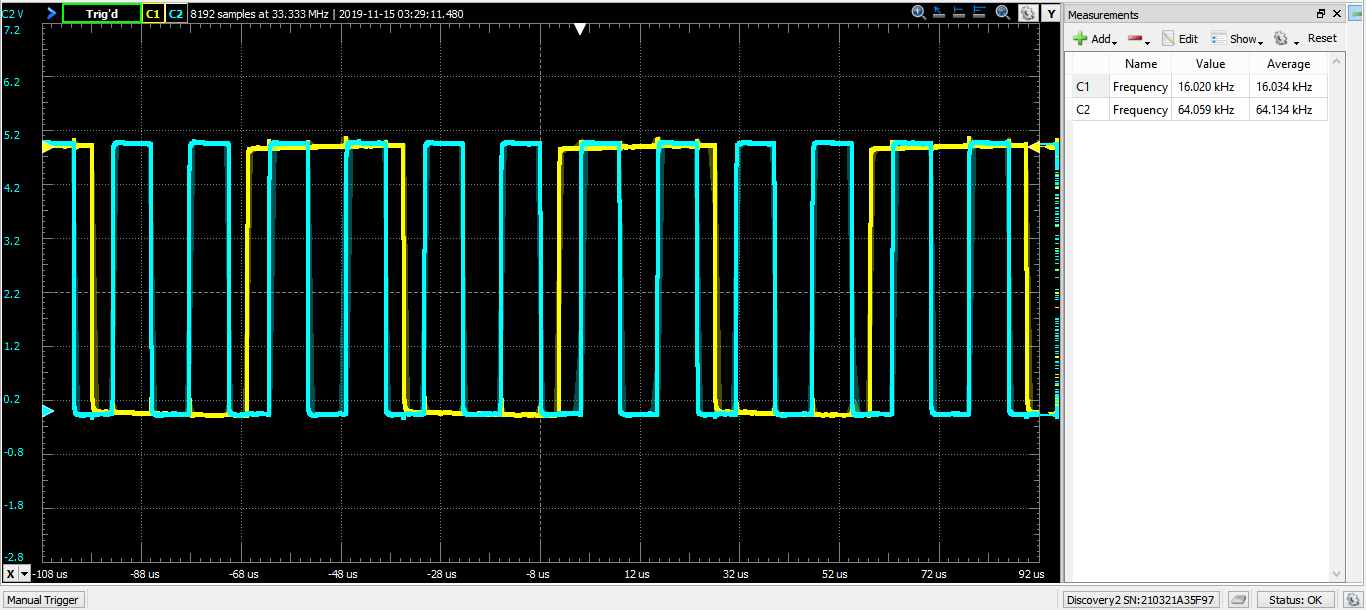
\includegraphics[width=\linewidth]{ImagenesOsciloscopio/SintetizadorFrecuencias1.PNG}
	\caption{La frecuencia sintetizada (azul) es 4 veces mayor que su referencia de $16KHz$(amarillo)}
	\label{sintetizadas}
\end{figure}

\subsubsection{Diseño}
Una de las formas más sencillas de generar un divisor de frecuencia es mediante el uso de dispositivos tipo \emph{Flip-Flop} en cascada. Sin embargo cuentan con la desventaja de solo poder dividir frecuencias mediante potencias de 2.
Se decidió utilizar un contador \textit{CD-4017} con el fin de dividir la frecuencia de la señal de entrada hasta 10 veces. No obstante, este circuito integrado, solo es capaz de contar y emitir flancos  cada vez que incrementa en 1 su contador. Por lo tanto debimos emplear un 
\emph{CD-4013} que nos provee Flip-Flops tipo D con el fin de obtener una señal con Duty-Cycle del 50\%. Debemos tener en cuenta los Flip-Flops son utilizados como divisores de clock en aplicaciones de electrónica digital. Por lo tanto obtendremos una señal con un periodo $2N$ con $N$ siendo la división de frecuencia que realiza el contador) mayor que el de la oscilación de referencia.
Otra alternativa al uso del Flip-Flop, y conservando al posibiliadad de dividir frecuencias por números no pares, es utilizar el comparador número de 2. Este comparador tiene la particularidad de operar sobre los flancos positivos de la señal de entrada. Por lo tanto, es posible acoplar la salida del contador directamente hacia la entrada del comparador II.

Para finalizar con esta sección, cabe destacar que al utilizar un contador como medio principal de divisor de frecuencia, es posible variar $N$ mediante conexiones sencillas entre las terminales del mismo.
\begin{figure}[H]
	\centering
	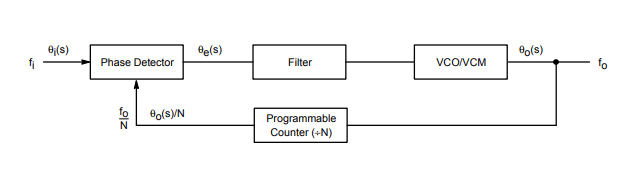
\includegraphics[width=\linewidth]{ImagenesVarias/PLLblockDiagram2.PNG}
	\caption{Diagrama en bloques del sintetizador de frecuencias}
	\label{blockdiagramfreqsynth}
\end{figure}


\begin{figure}[H]
	\centering
	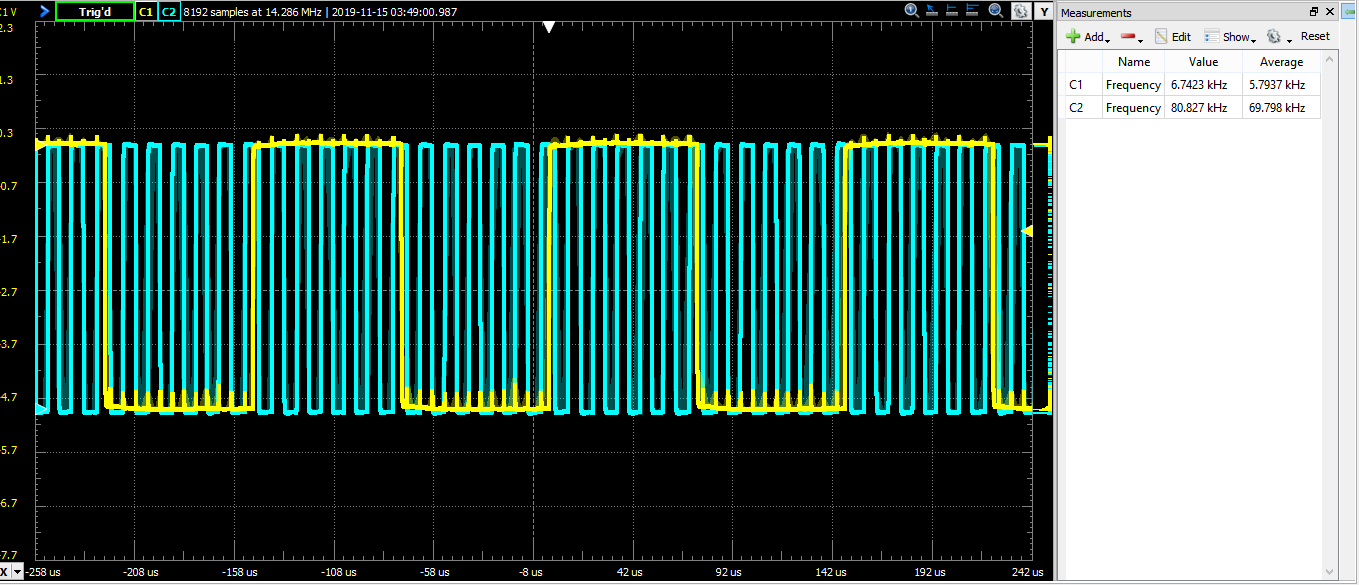
\includegraphics[width=\linewidth]{ImagenesOsciloscopio/SintetizadorFrecuencias3.PNG}
	\caption{Multiplicación de frecuencia en 12 veces}
	\label{freqsynth12}
\end{figure}


\subsubsection{Demodulación FM con PLL}
Una señal modulada en frecuencia se caracteriza por mostrar cambios en su frecuencia a lo largo del tiempo. En estos cambios es donde se aloja la información que se desea transmitir, llamada moduladora.

\begin{figure}[H]
	\centering
	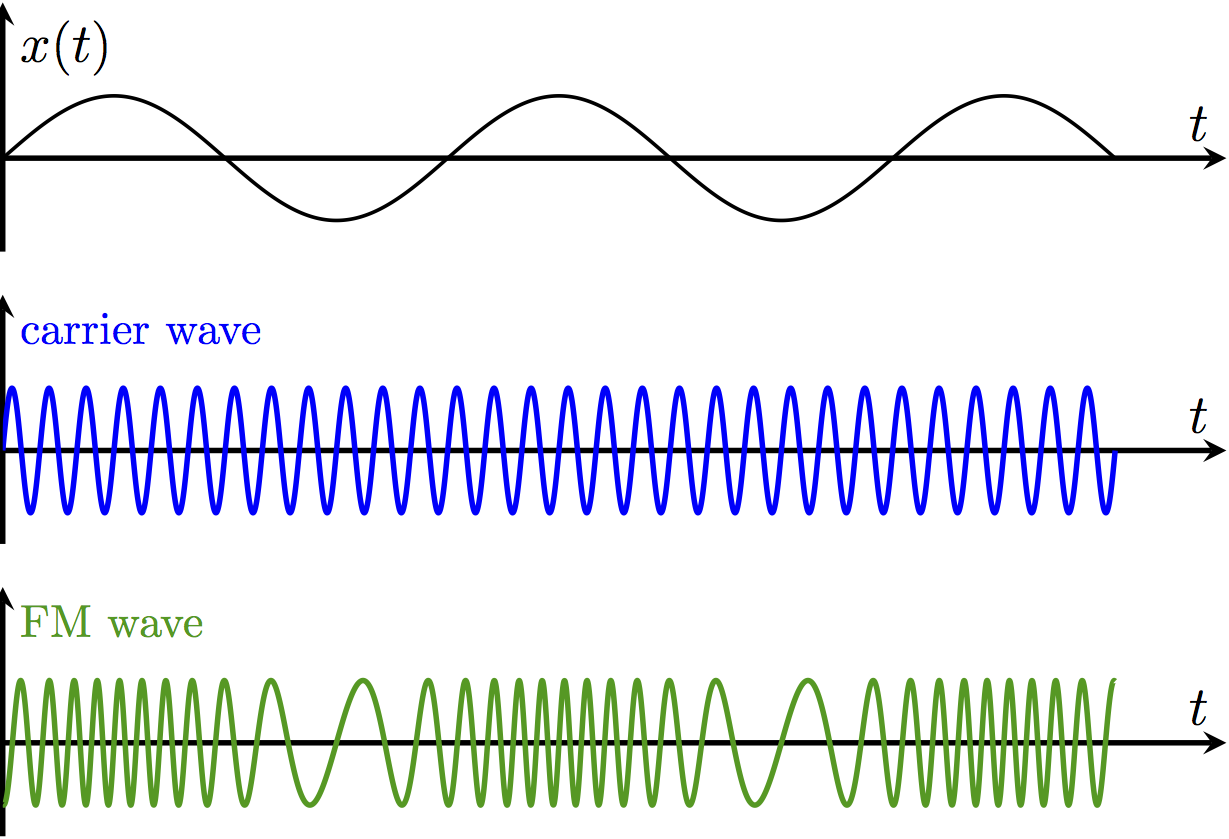
\includegraphics[scale=0.5]{ImagenesVarias/FMmodulation1.png}
	\caption{Modulación en frecuencia}
	\label{freqmod1}
\end{figure}

Luego la señal modulada es transmitida hacia el pin de entrada del PLL. Es importante tener en cuenta que la frecuencia de la señal modulada debe mantenerse dentro de los limites de operación, es decir no desengancharse ni tener frecuencias mayores a las que el VCO puede proveer.

Una vez recibida sera comparada con la oscilación libre del VCO. El comparador emitirá una señal de error con una energía proporcional a la diferencia en frecuencia. Es por es que aquellas zonas donde la frecuencia de la señal modulada es más alta, más energía aportara a la entrada del VCO.

\begin{figure}[H]
	\centering
	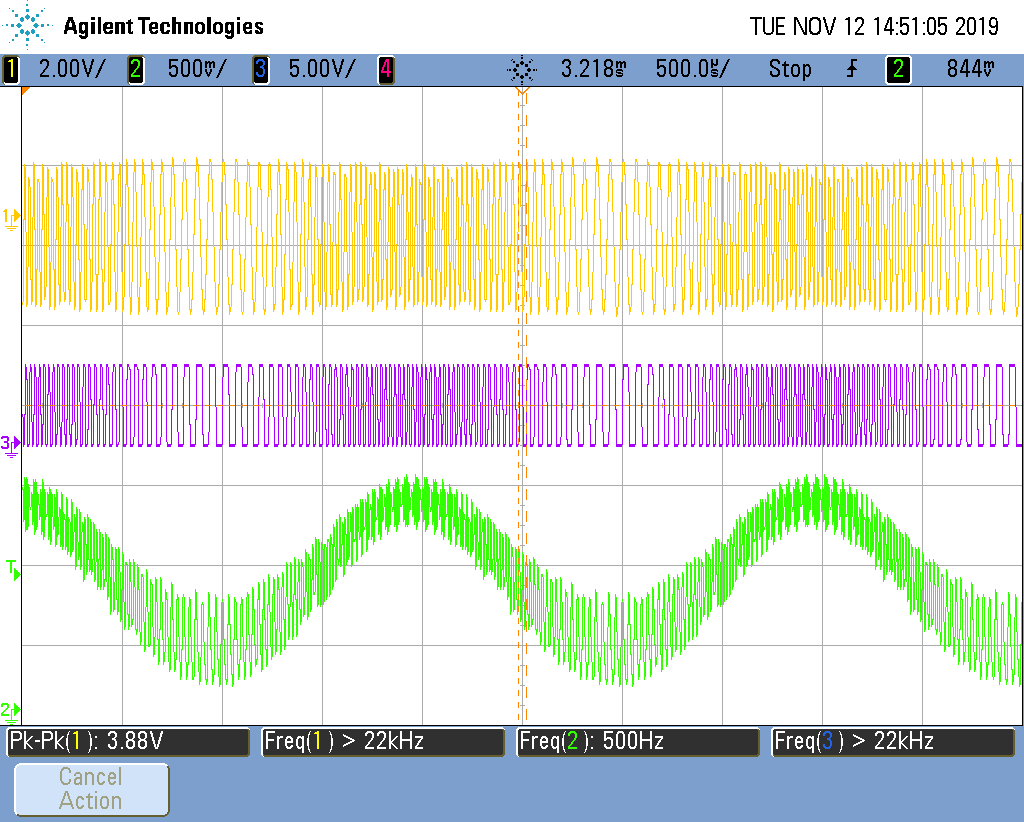
\includegraphics[scale=0.5]{ImagenesOsciloscopio/Demodulacion.png}
	\caption{Demodulación FM}
	\label{freqdemod0}
\end{figure}

Como se puede apreciar en la figura \ref{freqdemod0}, aquellas zonas dónde la frecuencia es mayor aportan mayor energía a la señal de error. Luego de ser filtrada por un filtro pasabajos obtenemos la señal demodulada.
\begin{figure}[H]
	\centering
	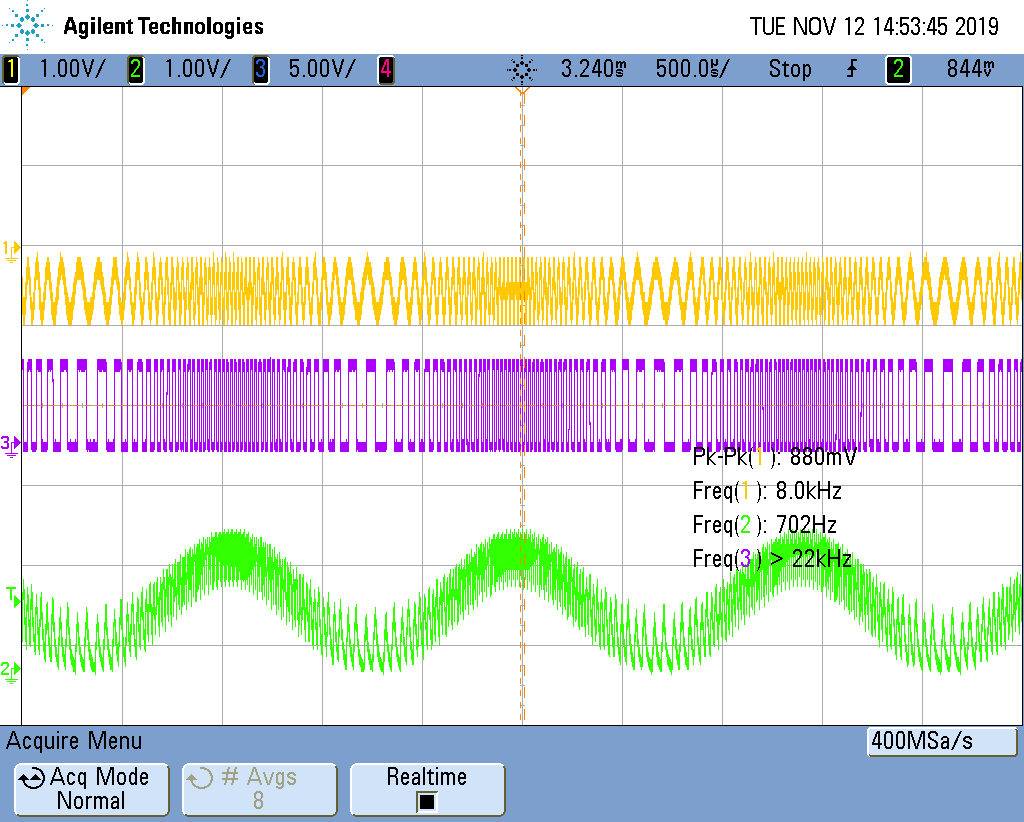
\includegraphics[scale=0.5]{ImagenesOsciloscopio/Demodulacion2.png}
	\caption{Demodulación FM}
	\label{freqdemod1}
\end{figure}

\begin{figure}[H]
	\centering
	\includegraphics[scale=0.5]{ImagenesOsciloscopio/Demodulacion3.png}
	\caption{Demodulación FM}
	\label{freqdemod2}
\end{figure}


\begin{figure}[H]
	\centering
	\includegraphics[scale=0.5]{ImagenesOsciloscopio/DemodulacionTriangular.png}
	\caption{Demodulación de onda triangular FM. Notese como la rama de subida de la triangular coincide con la zona de mayor densidad en la señal amarilla(entrada)}
	\label{freqdemodtrian}
\end{figure}

\subsubsection{Tiempos de establecimiento}
\underline{Filtro RC}
\begin{figure}[H]
	\centering
	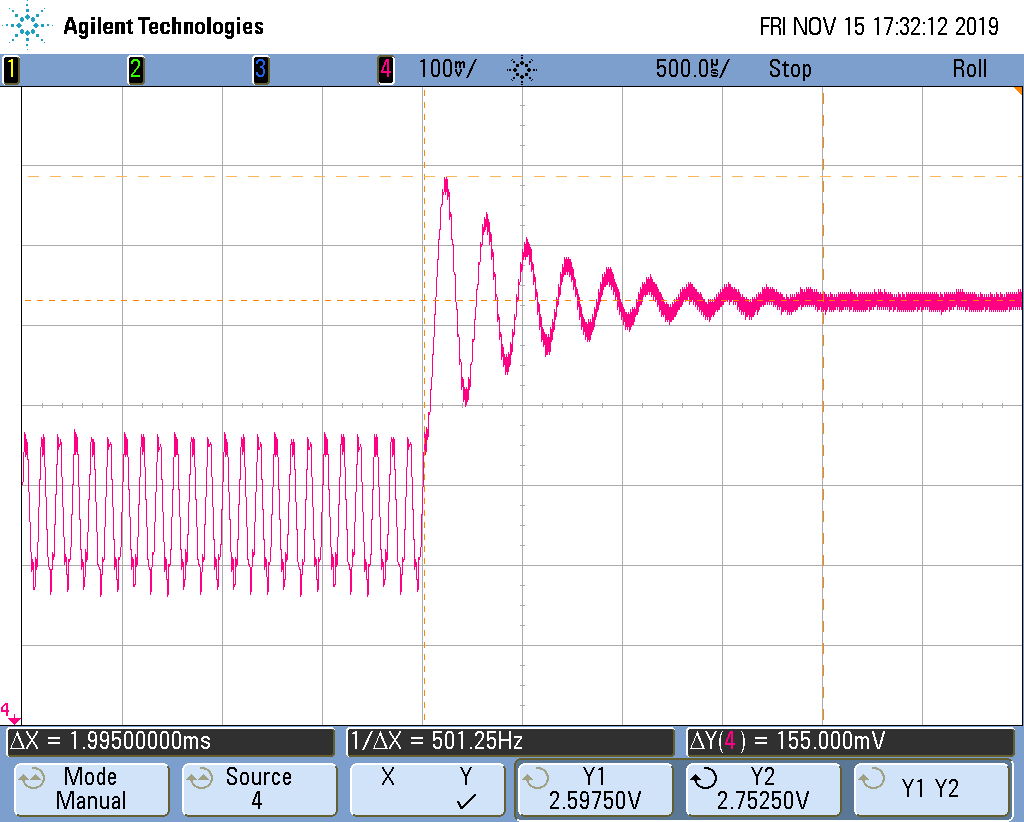
\includegraphics[scale=0.5]{ImagenesOsciloscopio/EscalonRCcomun.png}
	\caption{Salto de frecuencia}
	\label{jump1}
\end{figure}
\underline{Filtro RC compensado}
\begin{figure}[H]
	\centering
	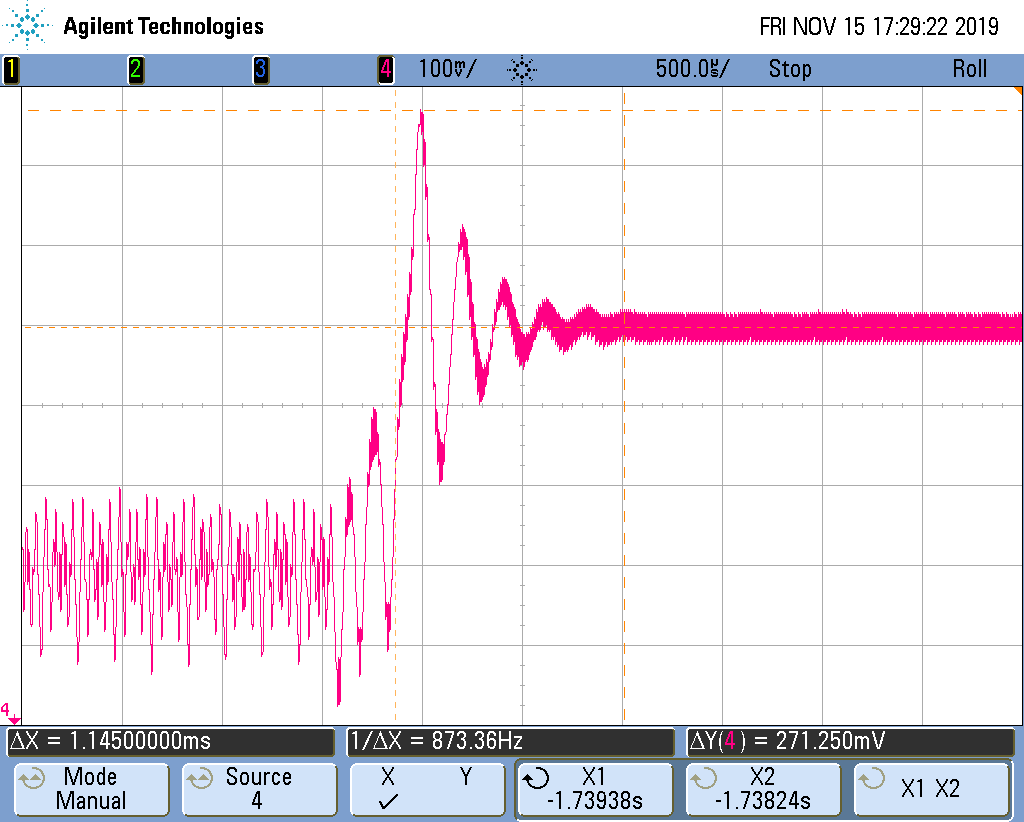
\includegraphics[scale=0.5]{ImagenesOsciloscopio/EscalonRCcompensado.png}
	\caption{Salto de frecuencia}
	\label{jump2}
\end{figure}


\subsubsection{Conclusiones}
El integrado \textit{CD-4046} demostró ser un circuito integrado muy versátil. Para maximizar la eficacia del diseño es conveniente comenzar por la calibración del VCO para luego trabajar con el LPF del lazo de realimentación. Es de suma importancia saber la antigüedad de los componentes en el mercado dado que la sobrecarga de datos puede llevar al usuario a utilizar información errónea. 



%Notas
%

%https://sites.google.com/site/ccolonelec101/wentworth-institute-of-technology/electronic-design/phase-lock-loop